\documentclass[16pt]{article}
\usepackage[margin=0.7in]{geometry} 
\usepackage{amsmath, amsthm, amssymb, mathrsfs, graphicx, mathtools, tikz, hyperref, enumitem}
\usetikzlibrary{positioning}
\newcommand{\n}{\mathbb{N}}
\newcommand{\z}{\mathbb{Z}}
\newcommand{\q}{\mathbb{Q}}
\newcommand{\cx}{\mathbb{C}}
\newcommand{\real}{\mathbb{R}}
\newcommand{\field}{\mathbb{F}}
\newcommand{\ita}[1]{\textit{#1}}
\newcommand{\com}[2]{#1\backslash#2}
\newcommand{\oneton}{\{1,2,3,...,n\}}
\newcommand\idea[1]{\begin{gather*}#1\end{gather*}}
\newcommand\ef{\ita{f} }
\newcommand\eff{\ita{f}}
\newcommand\proofs[1]{\begin{proof}#1\end{proof}}
\newcommand\inv[1]{#1^{-1}}
\newcommand\setb[1]{\{#1\}}
\newcommand\en{\ita{n }}
\newcommand{\vbrack}[1]{\langle #1\rangle}
\newenvironment{theorem}[2][Theorem]{\begin{trivlist}
\item[\hskip \labelsep {\bfseries #1}\hskip \labelsep {\bfseries #2.}]}{\end{trivlist}}
\newenvironment{lemma}[2][Lemma]{\begin{trivlist}
\item[\hskip \labelsep {\bfseries #1}\hskip \labelsep {\bfseries #2.}]}{\end{trivlist}}
\newenvironment{exercise}[2][Exercise]{\begin{trivlist}
\item[\hskip \labelsep {\bfseries #1}\hskip \labelsep {\bfseries #2.}]}{\end{trivlist}}
\newenvironment{reflection}[2][Reflection]{\begin{trivlist}
\item[\hskip \labelsep {\bfseries #1}\hskip \labelsep {\bfseries #2.}]}{\end{trivlist}}
\newenvironment{proposition}[2][Proposition]{\begin{trivlist}
\item[\hskip \labelsep {\bfseries #1}\hskip \labelsep {\bfseries #2.}]}{\end{trivlist}}
\newenvironment{corollary}[2][Corollary]{\begin{trivlist}
\item[\hskip \labelsep {\bfseries #1}\hskip \labelsep {\bfseries #2.}]}{\end{trivlist}}
\hypersetup{colorlinks, linkcolor=blue}

\newcounter{itemnumber}

\begin{document}
\large
\date{}
\title{\Large Assignment 5 Part 1 \\ Ryan Heffelman \\ March 27^\(th\), 2024 \\ MTH 1240 \\ Sara Jensen}
\maketitle
    \begin{enumerate}
        \item[\textbf{Problem 1.}] A, C, B, D
        \item[\textbf{Problem 2.}]
        \item[Plurality:] A, B, C
        \item[Copeland's:] B, C, A
        \item[IRV:] A, B, C
        \item[\textbf{Problem 3.}]
        \item[1.] 67 yes votes.
        \item[2.] 34 yes votes. This happens when there are 51 senators present (smallest integer that's more than half of 100). For a vote to pass you need at least two-thirds yes votes. \(51 \cdot \frac{2}{3} = 34\). 34 is at least two-thirds yes votes.
        \item[3.] I didn't want to bother editing your tiny resolution plot, please forgive me, please accept my spreadsheet recreation (Figure 1).
        \item[4.] It would go down on the y-axis and to the right on the x-axis. So a down-right motion. This operation would change the outcome in the cases of cells (0, 6), (3, 4), and (4, x) where x \(>\) 3.
        \item[5.] It would go right on the x-axis, decrementing the amount of people present and not changing the amount of people who said yes. It would change the outcome in cells (4, x) where x \(>\) 3.
        \begin{figure}
            \centering
            \caption{}
            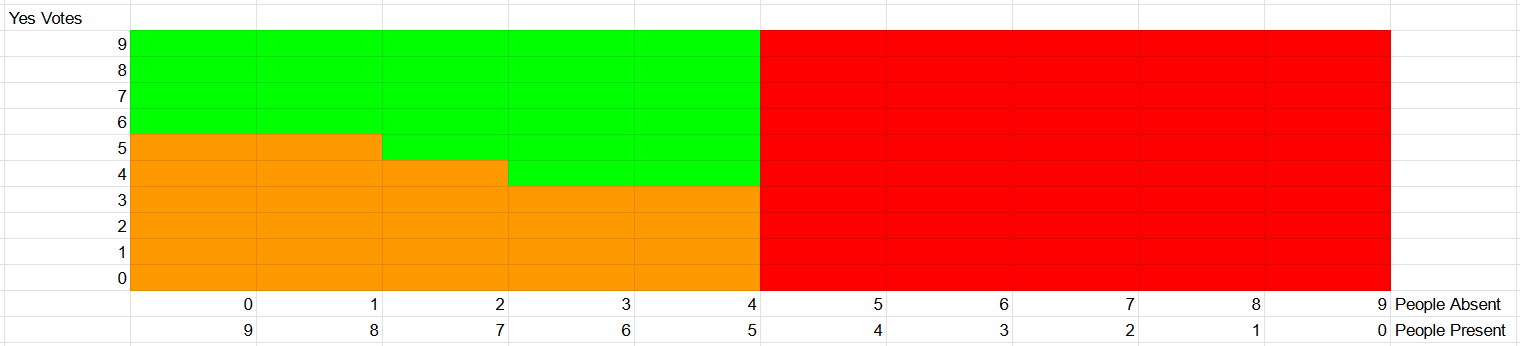
\includegraphics[width=1\linewidth]{image.png}
            \label{Figure 1}
        \end{figure}
        \item[\textbf{Problem 4.}]
        \begin{enumerate}
            \item[1.] It meets the majority criterion. A majority candidate would have more than all of the other candidates combined, thus they could never be eliminated, and in the final round, even in the worst case scenario for the majority candidate, they would have more than the other candidate.
            
            \item[2.] It does not meet the IIA. Isn't that the whole thing behind Arrow's impossibility theorem? Figure 2 is my example, by default C wins under IRV, but if you take out the loser A, C is our first round elimination. For the record I got this example from: https://mathbooks.unl.edu/Contemporary/sec-5-5-arrow.html 

            \item[3.] I'm pretty sure the answer is yes, but I don't really have a great explanation for it. If all voters prefer A over B, then B cannot exist in a row that is higher or equally as high as A's highest row. For example, if A is in the highest row, B cannot be in the highest row, so it makes sense that B would have to be eliminated after A.

            \item[4.] IRV does not meet the Condorcet condition. Figure 2 shows that, D is a condorcet winner, but as previously established C wins by default.

            \item[P.S.] I might just be a bad student or inattentive, but I swear I don't recall some of this stuff being gone over. I'm not sure how I was supposed to know what the IIA is or the pareto condition outside of googling. Also the document says "Due May 2" and it is not due May 2nd.
            \end{enumerate}
            
        
    \end{enumerate}
    \begin{figure}
            \centering
            \caption{}
            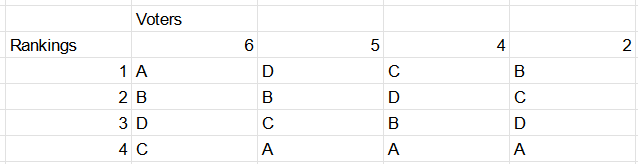
\includegraphics[width=1\linewidth]{image2.png}
            \label{Figure 2}
        \end{figure}
\end{document}